
\section{CLIC Overview}

\subsection{The Architecture of CLIC}

To address the above challenges in cross-platform computing, CLIC is designed as a cloud-native framework with a Graphic Convolutional Network (GCN) model for hardware-conscious platform selection.
Figure~\ref{fig:architecture} demonstrates the architecture of CLIC, which consists of three layers. 



\begin{figure}[tbh]
  \centering
  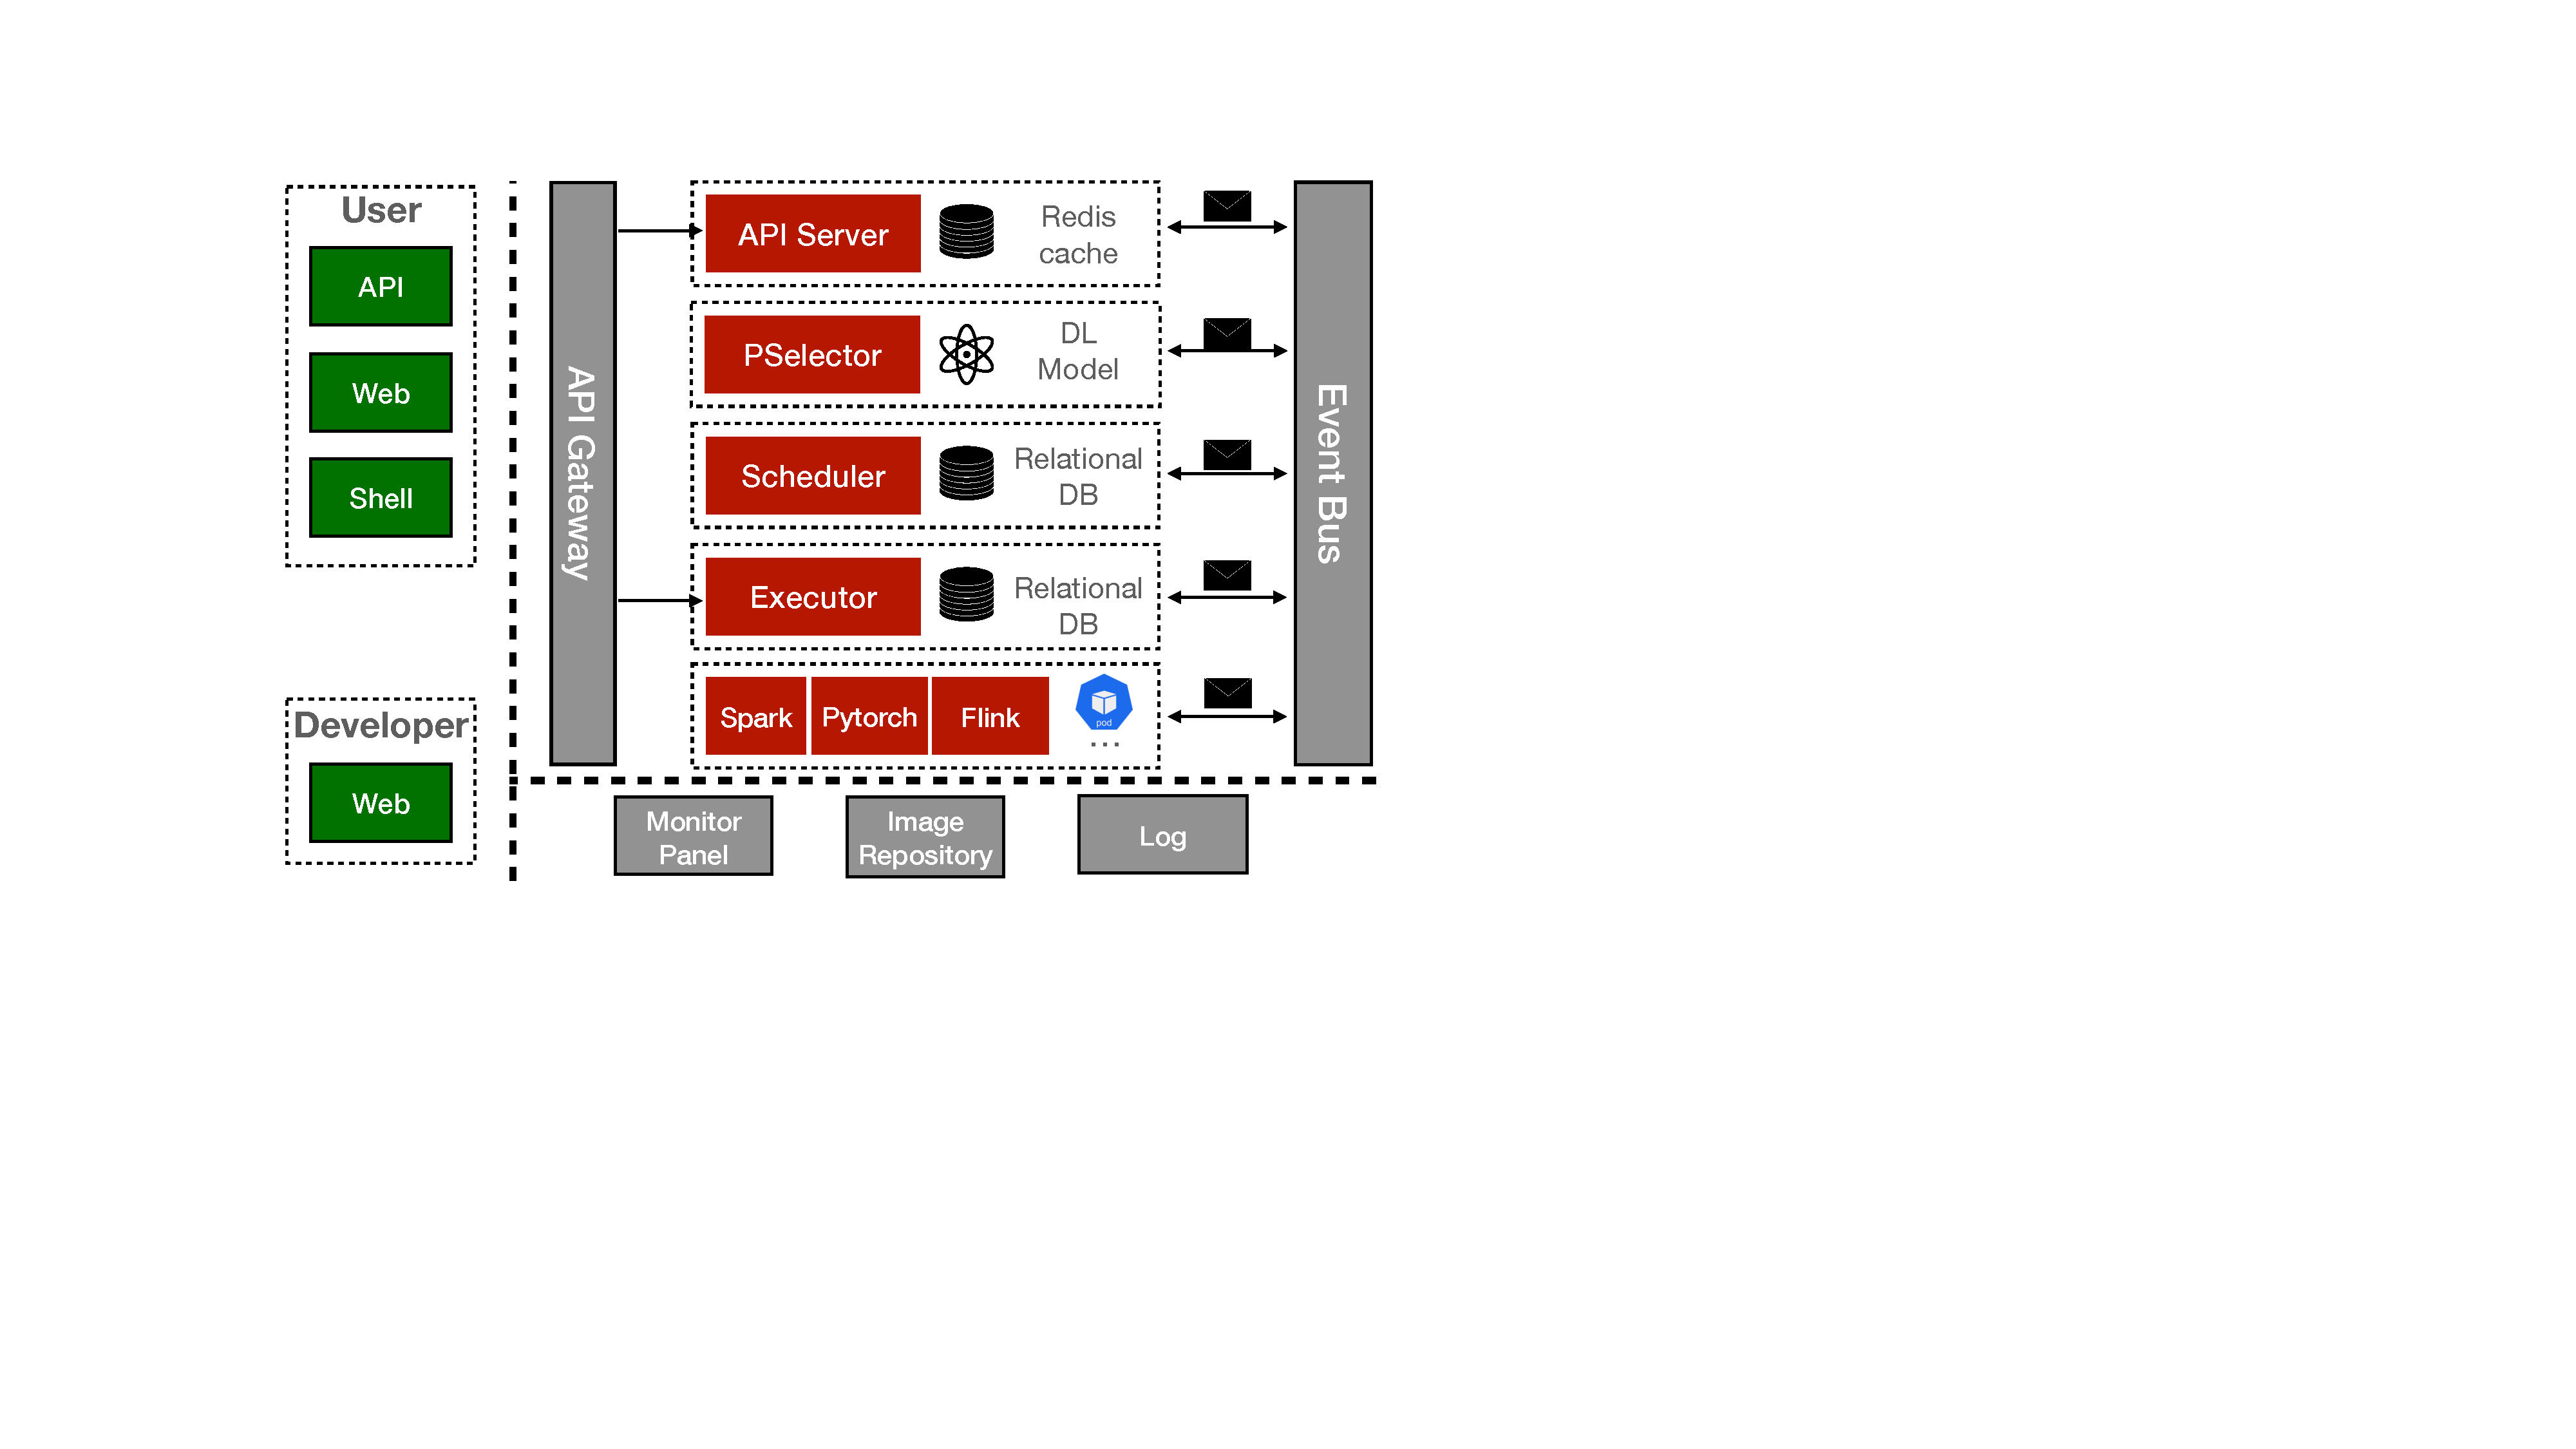
\includegraphics[width=0.8\linewidth]{figures/CLIC-arch-2.pdf}
  \caption{The architecture of CLIC}
  \label{fig:architecture}
\end{figure}

\textbf{1) Abstraction} CLIC provides a high level abstraction of a workflow, which uses platform independent logical operators to express the computation tasks in the workflow. A logical operator is a baisc functional unit, that describes only the computation semantics like functionality, parameter list, etc.. 
After hardware-conscious platform selection that aims at optimizing the overall workflow efficiency, each logical operator is assigned with a data processing platform and becomes a physical operator. 
Since different platforms CLIC supports data models of the corresponding platforms and provides data transfer operators that automatically match the input and output data formats of adjacent operators.
By assigning operator platforms, adding model translaters, and merging adjacent nodes of the same platform as one job, CLIC reconstructs the logical workflow as a physical workflow.
To facilitate development, CLIC provides a set of logical operators and corresponding implementations in mulitple corresponding data processing platforms.
Developers and data scientists can directly utilize these operators to construct their workflow, while new operators and platforms can also be flexibily integrated.


***data model conversion operator?***
 
\textbf{2. Service-Based Framework} To fully utilize features of cloud, CLIC embrace microservices, where each functional module is designed as a microservice, such as Executor, Scheduler, and Optimizer.
Microservices enable flexibility where each module can be devleoped, tested and deployed independently.
Specifically, domain specific functionalities such as optimizers can be developed with its own data storage and programming platform, which makes the system highly extensible to integrate new optimization schemes.
The CLIC server consists of a publish/subscribe mode event bus. All the microservices interact with each other by publishing and subscribing to a specific channel in the event bus. The main microservices are as follows.

The main microservices are as follows. a) \textit{API Server} receives the API call from clients and responds to it whenver the result is ready. For example, when receiving a configuration lookup request, it publishs the event to the specific channel and starts to listen. After receiving the result ready event, it wraps the result with headers and responses to the client. At last, we use redis database to cache some of the query result to speed up the process.
b) \textit{PSelector} takes a logical plan as input and outputs a physical plan whose operator is assigned a platform. Inside the PSelector, it utilizes the prementioned GNN model to determine the platform. We detailedly describe the approach in Section 4. Thanks to the microservice architecture, the model can be easily updated or replaced at runtime. c) \textit{Scheduler} records the status of all resources and specifies the number of container instances and the targeted nodes to be deployed etc.. The resource status are periodically retreived from Executor and maintained in the Scheduler's database. Again different scheduling policies can be developed as independent microservices and deployed according to requirements.
d) \textit{Executor} controls the underlying container resources using the Kubernetes API and submits the jobs to them. The controlment includs instantiating, pausing, destroying the container and restarting jobs whenever it fails. All the platform-related configuration files like container and network are declared in the form of YAML and managed by Helm~\cite{} charts and passed to the deployed platforms in execution.
The four core components of CLIC are developed and deployed independently, making CLIC a flexible system with high availability.



\textbf{3. Cloud-Native Task Deployment} Besides designing the cloud-native framework, CLIC decouple data processing platforms from the framework to facilitate extensible platform integration and independent deployment.
In this way, all physical operators of a platform are built as a container image, thus each platform is developed and maintained independently.
Moreover, one platform of different versions can be kept as separate images to provide backward compatibility.

After platform selection, each task in a workflow is associated with an image of its corresponding platform.
CLIC merges adjacent tasks of the same platform to optimize data transfer costs, and tasks of different platforms are launched as separate instances.
To execute one or multiple adjacent physical operator, a platform image contains a driver program to drive the workflow execution. In the deployment of a platform image, Executor passes the operators information to the driver program who interprets and calls the corresponding operators one by one.






\iffalse
\textbf{Platform-agnostic Programming}   We thin wrap each integrated platform's API to offer a logical operator set and provide various data models like the vector/matrix in linear algebra. The logical operator describes only the computation semantics like functionality, parameter list, etc.. User can build platform-agnostic workflow using the logical operator set and data models, and run it on any (integrated) platform. This greatly alleviates users burden of struggling in the overwhelming platforms.

\textbf{Cross-platform Computing}        To support building the cross-platform workflow, we (i)offer corresponding logical operator sets and data models for different computing paradigms, and (ii)implement a series of data model conversion and data transmission operators to bridge operators from two paradigm. For example, to support both relational and linear algebra we first provide relational operators along with its table model as well as linear operators along with its vector/matrix models, and then implement a conversion operator that assigns each column a name(column number) and a data type to transform a matirx to table.

\textbf{Automatic Platform Selecting}    CLIC can automatically convert the logical plan to the physical plan, i.e. select a platform for each logical operator. To achieve this, we introduce an end-to-end GNN-based model that takes as input a logical plan and outputs the platform-specific physical plan that has the lowest cost. Each logical operator in the logical plan is vectorized using our novel feature extraction method.

\textbf{High Availability}               The high availability is ensured by (i) status monitor, (ii) container self-healing mechanism and (iii) data recovery. With the help of ZooKeeper, we implement health check and progress reportor to monitor the status of the running jobs. When the job fails, CLIC will instantiate a new container and restart the job using Kubernetes self-healing mechanism. The input data is recorverd from checkpoints that are implicitly inserted (by the Planbuilder ?).

\textbf{Agile Integration}               We containerized each platform along with its neccessary components like the above progress reportor, so that dependency management and environment setup should be a lot easier. What's more, we apply semantic versioning on the integrated platforms to avoid conflicts like expired API call after iterate updates. Apart from that, thanks to the feature extraction method, the GNN-model doesn't need to be retrained whenver there's a newly operator/platform anymore, i.e. is compatible for an integration.

%\subsection{CLIC Architecture} 
Figure \ref{fig:architecture} demonstrates the architecture of CLIC that consists of the clients(left), the CLIC server(right top), and 3rd-party services.

\textbf{Client}  There're two types of clients for different roles: user and developer. The user programmes the workflow using clients like native lanuage API, Web interface or command line. The user client wraps the workflow with headers and sends to the CLIC API server for execution. The developer client is a developer toolkit for registering configuration, observe and manage the cluser, etc.

The CLIC server consists of a series of microservices and a publish/subscribe mode event bus. All the microservices interact with each other by publishing and subscribing to a specific channel in the event bus. The main microservices are as follows:

\textbf{API Server}  The API Server receives the API call from clients and respondes to it whenver the result is ready. For example, when receiving a configuration lookup request, it publishs the event to the specific channel and starts to listen. After receiving the result ready event, it wraps the result with headers and responses to the client. At last, we use redis database to cache some of the query result to speed up the process.

\textbf{PSelector}   PSelector takes a logical plan as input and outputs a physical plan whose operator is assigned a platform. Inside the PSelector, it utilizes the prementioned GNN model to determine the platform. Notice that, the GNN can also be replaced by other models like ML-based models or heuristic methods as long as their input format is aligned.

\textbf{Scheduler}   The Scheduler specifies the number of container instances, target nodes etc. given the current resource utilization. The resource status are periodically retreived from Executor and maintained in the Scheduler's database.

\textbf{Executor}    The Executor controls the underlying container resources using the Kubernetes API and submits the jobs to them. The controlment includs instantiating, pausing, destroying the container and restarting jobs whenever it fails. All the platform-related configuration files like container and network are declared in the form of YAML and managed by Helm charts.
\fi

% We propose CLIC, a highly extensible cloud-native framework for cross-platform computing. To address the above challenges, we decouple data processing platforms from the underlying framework to facilitate independent development and deployment.
% CLIC divides a workflow into multiple \textit{tasks} where adjacent tasks belong to different platforms and are launched as separate instances.
% To express cross-platform workflows, CLIC uses \textit{logical operators} as the abstraction, where each logical operator describes a minimal functional unit.
% A \textit{physical operator} is the implementation of a logical operator on a specific platform, thus there may exist a one-to-many mapping between a logical operator and multiple physical operators.
% With all physical operators of a platform being built as a container image, each task in a workflow is associated with an image of its corresponding platform. This design enables agile platform integration where new platforms can be developed and integrated in a plug-and-play mode, without rebuilding the entire framework. By maintaining platforms with diverse versions and system configurations with images, CLIC provides backward platform compatibility and consistent performance. 
% The architecture of CLIC helps maintain independent development and deployment environments.

%To enable dynamic scaling in a workflow, we implement a scheduler to specify needed resources for each task at runtime.




\iffalse
Figure \ref{fig:architecture} demonstrates the architecture of CLIC, which consists of four major microservices, i.e., PlanBuilder, Optimizer, PSelector, and Scheduler. PlanBuilder provides the information of logical operators to build the \textit{logical plan} of a workflow (step 1). The logical plan is sent to Optimizer for potential optimizations, and then sent to PSelector to assign platforms by mapping \textit{logical operators} to \textit{physical operators} with a GCN model (step 2). The output of PSelector is the \textit{physical plan}, which is used by Scheduler to deploy corresponding tasks on the cloud. 
When the physical plan of a workflow arrives, Scheduler launches instances of the selected platforms subsequently and scales them according to workloads (step 4). An instance of a platform contains an Executor that receives and translates the physical plan from Scheduler and calls the specified physical operators. Deploying a workflow with multiple tasks requires monitoring their running states of tasks. As shown in the figure, Executor regularly sends heart-beats with its running states to Scheduler. It is worth noting that, to support QoS requirements of various workflows, Scheduler provides interfaces to develop different resource allocation schemes for flexible scaling.
\fi

\iffalse
In CLIC, adjacent operators that run on the same platform are deployed as one Kubernetes task. We store physical operators developed on a platform (a specific version) as a container image. It contains all physical operator implementations and an Executor that translates the physical plan and executes the corresponding operators. Developers can build their own images after adding or re-implementing new operators on a platform. After updating the image information and corresponding operator mappings in the configuration server, developers can run workflows with their newly developed platforms and operators without affecting other workflows. In this way, CLIC enables flexibility in both development and deployment, which fits for the requirements of data science applications.

CLIC is a cloud-native computing framework designed for cross-platform data science workflows. CLIC integrates platforms from various domains and provides a consistent programming model, including multiple data models and algebras. CLIC selects platforms for a given workflow using GCN to optimize the overall performance. What’s more, CLIC enables passing UDF and dynamic control flow for building advanced workflow. Last but not the least, CLIC encapsulates components as containerized \textit{Microservices} and deploy them on the Kubernetes.

In order to integrate multiple platforms and offer a unified programming model, CLIC decouples the operator’s semantic and execution to the logical operator and the physical operator. The logical operator is used for declaring a workflow. It only describes the properties like the parameter list, return value, etc. and is not associated with any platform; The physical operator is the corresponding executable implementation on a specific platform. The mapping relationship between the logical and physical operator is 1-n. Programmers can construct the workflow using only logical operators without knowing the underlying platforms and CLIC can improve workflow performance by selecting the best physical operators.

The PlanBuilder offers data scientists multiple data models and logical operators to build the workflow. The provided data models including table, vector, matrix and graph, and the provided logical operators including various algebraic operations, data model conversion algorithms, and control flow primitives. The Planbuilder organizes the workflow as a DAG form logical plan composed of logical operators and their dependencies (step 1). The logical plan is then sent to the Middleware.

The Middleware contains a SQL parser, several optimization rules, and the GCN, which optimize the logical plan and determine physical operators (step 2). It returns the optimized logical plan to the PlanBuilder. After that, the adjacent logical operators bound to the same platform are grouped as sub-logical-plans and sent to the Scheduler (step 3). 

Scheduler is responsible for multi-task scheduling. It manages all workflows’ running states in the configuration server, as well as other meta information such as platform configurations, logical/physical operator properties, the operator mapping table, etc. When a new logical plan arrives, the Scheduler starts a specific number of instances of the determined platform based on workloads and sends the logical plan (step 4). 
\fi


% \begin{figure*}
%     \centering
%     \subfigure[Original logical plan]{
%         \label{fig:dag1}
%         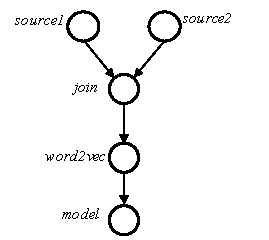
\includegraphics[width=0.18\textwidth]{figures/dag1.pdf}
%     } 
%     \subfigure[Optimized logical plan]{
%     \label{fig:dag2}
%         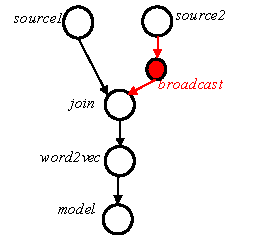
\includegraphics[width=0.18\textwidth]{figures/dag2.pdf}
%     } 
%     \subfigure[Platform selection]{
%     \label{fig:dag3}
%         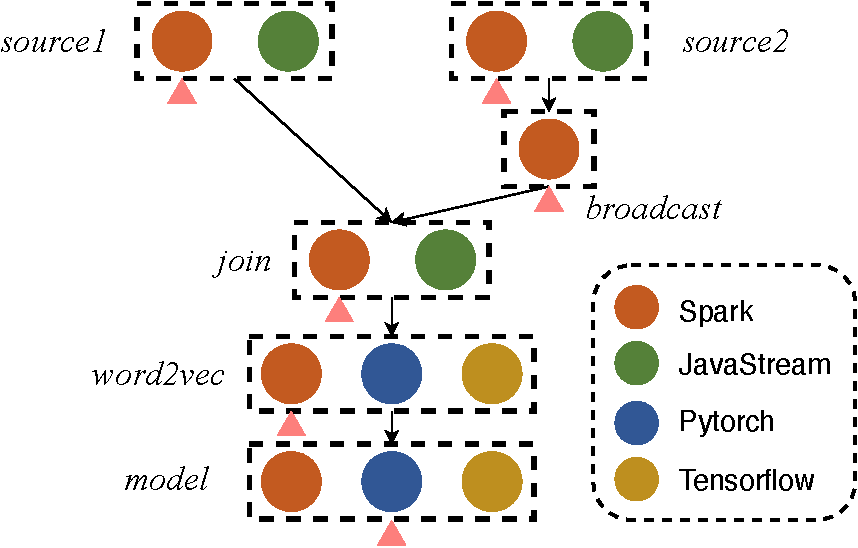
\includegraphics[width=0.27\textwidth]{figures/dag3.pdf}
%     }
%     \subfigure[Physical plan]{
%     \label{fig:dag4}
%         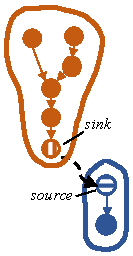
\includegraphics[width=0.1\textwidth]{figures/dag4.pdf}
%     }
%     \vspace{-5pt}
%     \caption{The case of running sentiment classification in CLIC}
%     \label{fig:optimizing-process}
%     \vspace{-5pt}
% \end{figure*}


\subsection{Case Study}
We adopt sentiment classification as a case to demonstrate how CLIC works. It is a common nature language processing task that classifies documents based on the semantics. The data processing tasks mainly include data ETL (Extract, Transforming, Loading) and training of a classification model. The pseudo-code of a simple implementation is shown in Listing \ref{code:workflow}.

\begin{listing}[ht]
\begin{minted}[frame=lines,
framesep=2mm,
baselinestretch=1.2,
fontsize=\footnotesize,
linenos]{python}
source1 = read('BBC-News.txt’)
source2 = read('Hamlet.txt')
corpus = join(clean_source1, clean_source2)

word_embedding = toMatrix(clean_corpus, Word2Vec)
    
model = Model('LSTM')
train(model, word_embedding['train'])
topic = test(model, word_embedding['test'])
\end{minted}
\caption{Pseudo-code of sentiment classification in CLIC}
\label{code:workflow}
\end{listing}
The processing steps are as follows. 1) Based on logical operators, PlanBuilder builds the logical plan for the workflow. As shown in Figure \ref{fig:dag1}, the logical plan is a  DAG consists of five logical operators. 2) Optimizer applies optimizations on the logical plan. In this case, because the data volume of \textit{source2} is way lesser than source1, CLIC implicitly inserts a \textit{broadcast} operator to put \textit{source2}’s data on all nodes in order to reduce communication times. The optimized logical plan is shown in Figure \ref{fig:dag2}. 3) Logical operators are assigned to platforms with a GCN model. Figure \ref{fig:dag3} shows the potential platforms of each logical operator and marks the selected platforms with red triangles. Two platforms are selected in this case, where model training is placed on Pytorch while the rest operators are assigned to Spark. 4) The adjacent Spark operators and the PyTorch operator are grouped into two tasks as shown in Figure \ref{fig:dag4}, because merging adjacent operators of the same platform as one task can mitigate data transfer overheads. Then Scheduler chooses the corresponding container images for the two tasks and deploys them on the cloud subsequently. Note that, in the generation of the physical plan, PlanBuilder implicitly inserts a \textit{sink} operator in Spark to output the intermediate results and a \textit{source} operator in Pytorch to read Spark’s results.
